\begin{problem}[20 pts \textbf{Exercise 5.2.6}]
    Let $f \in C(\mathbb{R}/\mathbb{Z}, \mathbb{C})$, and let $(f_n)_{n=1}^\infty$ be a sequence of functions in 
$C(\mathbb{R}/\mathbb{Z}; \mathbb{C})$.

\begin{enumerate}[(a)]
    \item Show that if $f_n$ converges uniformly to $f$, then $f_n$ also converges to $f$ in the $L^2$ metric.

    \item Give an example where $f_n$ converges to $f$ in the $L^2$ metric, but does \emph{not} converge to $f$ uniformly.
    \\
    \emph{(Hint: take $f = 0$. Try to make the functions $f_n$ large in sup norm.)}

    \item Give an example where $f_n$ converges to $f$ in the $L^2$ metric, but does \emph{not} converge to $f$ pointwise.
    \\
    \emph{(Hint: take $f = 0$. Try to make the functions $f_n$ large at one point.)}

    \item Give an example where $f_n$ converges to $f$ pointwise, but does \emph{not} converge to $f$ in the $L^2$ metric.
    \\
    \emph{(Hint: take $f = 0$. Try to make the functions $f_n$ large in $L^2$ norm.)}
\end{enumerate}
\end{problem}
\begin{proof}[proof of (a)]
  If \(f_n \to f\) uniformly, then for all \(\varepsilon > 0\), there exists \(N > 0\) s.t. \(\left\vert f_n(x) - f(x) \right\vert < \varepsilon  \) for all \(x \in [0, 1]\). Thus, 
  \begin{align*}
    \left\lVert f_n - f \right\rVert_2 &= \sqrt{\langle f_n - f, f_n - f \rangle } = \sqrt{\int _0^1 (f_n - f)(x) \overline{f_n - f}(x) \, \mathrm{d} x  } \\
    &= \sqrt{\int _0^1 \left\vert (f_n - f)(x) \right\vert^2 \, \mathrm{d} x} = \sqrt{\int _0^1 \left\vert f_n(x) - f(x) \right\vert^2 \, \mathrm{d} x  } < \sqrt{\int _0^1 \varepsilon ^2 \, \mathrm{d} x } = \varepsilon.     
  \end{align*}     
  This shows \(\lim_{n \to \infty} \lVert f_n - f \rVert_2 = 0  \), i.e. \(f_n\) also converges to \(f\) in the \(L^2\) metric.    
\end{proof}

\begin{proof}[proof of (b)]
  Let \(f(x) = 0\) and 
  \[
    f_n(x) = \begin{dcases}
      1 - nx, &\text{ if } 0 \le x \le \frac{1}{n} ;\\
      0, &\text{ if }  \frac{1}{n} < x \le 1.
    \end{dcases},
  \] 
  then we have 
  \begin{align*}
    \lVert f_n - f \rVert_2 &= \sqrt{\int _0^1 \left\vert f_n(x) \right\vert^2 \, \mathrm{d} x} = \sqrt{\int _0^{\frac{1}{n}} (1 - nx)^2 \, \mathrm{d} x} = \sqrt{\frac{1}{3n}} \to 0 \text{ as } n \to \infty.    
  \end{align*}
  Hence, \(f_n \to f\) in the \(L^2\) metric. However, suppose \(f_n \to f\) uniformly, then for \(\varepsilon = \frac{1}{3}\), there exists \(N > 0\) s.t. \(n \ge N\) implies 
  \[
    \left\vert f_n(x) - f(x) \right\vert = \left\vert f_n(x) \right\vert < \varepsilon = \frac{1}{3} \quad \forall x \in [0, 1] 
  \]      
  but \(f_n(0) = 1\) for all \(n\) and \(1 > \frac{1}{3}\), so this is impossible. Hence, \(f_n\) does not converge to \(f\) uniformly.   
\end{proof}

\begin{proof}[proof of (c)]
  We use the same \(f_n\) and \(f\) as in (b), then we have shown that \(f_n \to f\) in the \(L^2\) metric, and now if \(f_n \to f\) pointwise, then for \(x = 0\) and \(\varepsilon = \frac{1}{3}\), there exists \(N > 0\) s.t. \(n \ge N\) implies 
  \[
    1 = \left\vert f_n(0) - f(0) \right\vert < \varepsilon = \frac{1}{3},
  \]        
  which is impossible, so \(f_n\) does not converge to \(f\) pointwise.   
\end{proof}

\begin{proof}[proof of (d)]
  Let \(f(x) = 0\) and 
  \[
    f_n(x) = \begin{dcases}
      n^3 x, &\text{ if } 0 \le x \le \frac{1}{n} ;\\
      -n^3 \left( x - \frac{2}{n} \right) , &\text{ if } \frac{1}{n} < x \le \frac{2}{n} ;\\
      0, &\text{ if } \frac{2}{n} < x \le 1.
    \end{dcases}
  \] 
  Then, for all \(x \in (0, 1]\) and for all \(\varepsilon > 0\), we know there exists \(N > 0\) s.t. \(\frac{2}{N} < x\), and thus for all \(n \ge N\), we have \(\frac{2}{n} \le \frac{2}{N} < x\) and thus \(f_n(x) = 0\), which gives \(\vert f_n(x) - f(x) \vert < \varepsilon  \). As for \(x = 0\), since \(f_n(0) = 0\) for all \(n\), so \(\vert f_n(0) - f(0) \vert < \varepsilon  \) for all \(\varepsilon > 0\) and all \(n \ge 1\). Thus, we can conclude that \(f_n \to f\) pointwise. Now since 
  \begin{align*}
    \lVert f_n - f \rVert_2 &= \sqrt{\int _0^1 \vert f_n(x) \vert^2 \, \mathrm{d} x} = \sqrt{\int _0^{\frac{1}{n}} n^6 x^2 \, \mathrm{d} x + \int _{\frac{1}{n}}^{\frac{2}{n}} n^6 \left( x - \frac{2}{n} \right)^2 \, \mathrm{d} x   } \\
    &\ge \sqrt{\int _0^{\frac{1}{n}} n^6 x^2 \, \mathrm{d} x } = \sqrt{\frac{n^3}{3}} \to \infty \quad \text{as } n \to \infty, 
  \end{align*}             
  so we know \(f_n\) does not converge to \(f\) under \(L^2\) metric.   
\end{proof}

\begin{problem}[20 pts]
    Let $\{\phi_N\} : \mathbb{R} \to \mathbb{R}$ be a sequence of continuous, 
periodic functions on $\mathbb{R}$ (with period 1) which satisfy
\[
\int_0^{1} \phi_N(t)\,dt = 1
\qquad\text{and}\qquad
\int_0^{1} |\phi_N(t)|\,dt \le M < \infty
\]
for all $N \in \mathbb{N}$, and
\[
\lim_{N\to\infty} \int_{\delta}^{1 - \delta} |\phi_N(t)|\,dt = 0
\]
for each $0 < \delta < 1$.  

Suppose that $f : \mathbb{R} \to \mathbb{R}$ is continuous and periodic with period $1$.  
Prove that
\[
\lim_{N\to\infty} \int_0^{1} f(x - t)\,\phi_N(t)\,dt = f(x)
\]
uniformly for $x \in \mathbb{R}$.
\end{problem}

\begin{proof}
    It is suffices to show that 
    \[
        \left \vert \int_0^{1} f(x - t)\,\phi_N(t)\,dt - f(x) \right \vert \ \le \varepsilon \quad \text{when $N$ large enough} 
    \]
    Since 
    \[
        \int_0^{1} \phi_N(t)\,dt = 1,
    \]
    we can get
    \[
        f(x) = f(x) \int_0^{1} \phi_N(t)\,dt = \int_0^{1} f(x)\phi_N(t)\,dt,
    \]
    and hence 
    \[
        \begin{aligned}
        \left \vert \int_0^{1} f(x - t)\,\phi_N(t)\,dt - f(x) \right \vert 
        &= \left \vert \int_0^{1} f(x - t)\,\phi_N(t)\,dt - \int_0^{1} f(x)\phi_N(t)\,dt \right \vert\\
        &= \left \vert \int_0^{1} (f(x - t) - f(x))\phi_N(t)\,dt \right \vert
        \end{aligned}
    \]
    Since $f$ is continuous and 1-periodic, it is bounded and uniformly continuous, then we can let $K$ such that
    \[
        K = \sup_{x \in \mathbb{R}} \lvert f(x) \rvert < \infty 
    \]
    For fix $\varepsilon > 0$, since $f$ is uniformly continuous on $\mathbb{R}$, there exists $0 < \delta < \frac{1}{2}$ such that
    \[
        \lvert y-x \rvert \le \delta \implies \lvert f(y) - f(x) \rvert \le \frac{\varepsilon}{2M} 
    \]
    Then we can use triangular inequality,
    \[
        \begin{aligned}
        \left \vert \int_0^{1} f(x - t)\,\phi_N(t)\,dt - f(x) \right \vert & \le \left \vert \int_0^{\delta} (f(x - t) - f(x))\phi_N(t)\,dt \right \vert \\
        & + \left \vert \int_{\delta}^{1-\delta} (f(x - t) - f(x))\phi_N(t)\,dt \right \vert \\
        & + \left \vert \int_{1-\delta}^{1} (f(x - t) - f(x))\phi_N(t)\,dt \right \vert 
        \end{aligned}
    \]
    Then we discuss the upper bound of three parts of integrals, for first part,
    \[
    \begin{aligned}
    \left \vert \int_0^{\delta} (f(x - t) - f(x))\phi_N(t)\,dt \right \vert & \le 
    \int_{0}^{\delta} \left \vert (f(x - t) - f(x)) \right \vert \left \vert \phi_N(t) \right \vert\,dt \\
    &\le \int_0^{\delta} \frac{\varepsilon}{2M} \left \vert \phi_N(t) \right \vert\,dt \  \\
    &\le \frac{\varepsilon}{2M} \int_0^{1} \left \vert \phi_N(t) \right \vert\,dt \le \frac{\varepsilon}{2}
    \end{aligned}
    \]
    and for the second part,
    \[
    \begin{aligned}
    \left \vert \int_{\delta}^{1-\delta} (f(x - t) - f(x))\phi_N(t)\,dt \right \vert &\le
    \int_{\delta}^{1-\delta} \left \vert (f(x - t) - f(x)) \right \vert \left \vert \phi_N(t) \right \vert\,dt \\
    & \le \int_{\delta}^{1-\delta} (2K) \left \vert \phi_N(t) \right \vert\,dt \\
    & \le (2K) \int_{\delta}^{1-\delta}\left \vert \phi_N(t) \right \vert\,dt \to 0 \quad \text{when $N$ large enough.}
    \end{aligned}
    \]
    and for the last part,
    \[
    \begin{aligned}
    \left \vert \int_{1-\delta}^{1} (f(x - t) - f(x))\phi_N(t)\,dt \right \vert & \le 
    \int_{1-\delta}^{1} \left \vert (f(x - t) - f(x)) \right \vert \left \vert \phi_N(t) \right \vert\,dt \\
    &\le \int_{1-\delta}^{1} \left \vert (f(x - t) - f(x-1)) \right \vert \left \vert \phi_N(t) \right \vert\,dt \\
    &\le \int_{1-\delta}^{1} \frac{\varepsilon}{2M} \left \vert \phi_N(t) \right \vert\,dt \  \\
    &\le \frac{\varepsilon}{2M} \int_0^{1} \left \vert \phi_N(t) \right \vert\,dt \le \frac{\varepsilon}{2}
    \end{aligned}
    \]
    So we can conclude that,
    \[
    \left \vert \int_0^{1} f(x - t)\,\phi_N(t)\,dt - f(x) \right \vert \le \frac{\varepsilon}{2} + 0 + \frac{\varepsilon}{2} = \varepsilon, \quad \text{when $N$ large enough.}
    \]
    and hence 
    \[
    \lim_{N\to\infty} \int_0^{1} f(x - t)\,\phi_N(t)\,dt = f(x)
    \]
    uniformly for $x \in \mathbb{R}$.
\end{proof}

\begin{problem}[15pts \textbf{Exercise 5.2.3.}]
    If $f \in C(\mathbb{R}/\mathbb{Z};\mathbb{C})$ is a non-zero function,
show that 
\[
0 < \|f\|_{2} \;\le\; \|f\|_{\infty}.
\]

\noindent
Conversely, if $0 < A \le B$ are real numbers, show that there exists a non-zero
function $f \in C(\mathbb{R}/\mathbb{Z};\mathbb{C})$ such that 
\[
\|f\|_2 = A 
\qquad\text{and}\qquad
\|f\|_{\infty} = B.
\]

\noindent
\textit{(Hint: let $g$ be a non-constant non-negative real-valued function in 
$C(\mathbb{R}/\mathbb{Z};\mathbb{C})$, and consider functions of the form
$f=(c + d g)^{1/2}$ for some constant real numbers $c,d>0$.)}
\end{problem}
\begin{proof}
  Since \(f\) is a non-zero continuous function, so we know 
  \[
    \lVert f \rVert_2 = \sqrt{\int _0^1 \vert f(x) \vert^2 \, \mathrm{d} x} > 0,  
  \] 
  and since 
  \[
    \lVert f \rVert_{\infty } = \sup _{x \in [0, 1]} \vert f(x) \vert,   
  \]
  so we know 
  \[
    \lVert f \rVert_2 = \sqrt{\int _0^1 \vert f(x) \vert^2 \, \mathrm{d} x} \le \sqrt{\int _0^1 \lVert f \rVert_{\infty }^2 \, \mathrm{d} x   } = \sqrt{\lVert f \rVert_{\infty }^2  } = \vert f \vert_{\infty }.    
  \]
  Hence, we can conclude \(0 < \lVert f \rVert_2 \le \vert f \vert_{\infty }  \). Now we prove that for any \(0 < A \le B\) where \(A, B\) are real numbers, there exists \(f \in C(\mathbb{R} / \mathbb{Z} , \mathbb{C} )\) s.t. \(\lVert f \rVert_2 = A \) and \(\lVert f \rVert_{\infty } = B \). Suppose \(\delta = B^2 - A^2 \ge 0\), we pick positive \((M, \mu )\) pairs s.t. 
  \[
    M > \max \left\{ 2 \mu , \left( \frac{\delta}{A^2} + 1 \right)\mu   \right\}  
  \]        
  so that if we let 
  \[
    \begin{dcases}
      c = B^2 - \frac{M}{M - \mu }\delta  \\
      d = \frac{\delta }{M - \mu }
    \end{dcases}
  \]
  then we can show that \(c > 0\) and \(d \ge 0\). For \(d\), since \(\delta \ge 0\) and \(M > \mu \), so \(d \ge 0\). As for \(c\), if \(\delta = 0\), then \(c = B^2 > 0\), otherwise we have 
  \begin{align*}
    c &= B^2 - \frac{M}{M - \mu } \delta = B^2 - \left( 1 + \frac{\mu}{M - \mu } \right)\left( B^2 - A^2 \right) = B^2 \left( \frac{-\mu }{M - \mu } \right) + \left( 1 + \frac{\mu }{M - \mu } \right) A^2 \\
    &= A^2 + \left( A^2 - B^2 \right)\left( \frac{\mu}{M - \mu } \right) = A^2 - \frac{\delta \mu }{M - \mu } > A^2 - \frac{\delta \mu }{\left( \frac{\delta}{A^2} + 1 \right)\mu - \mu} = A^2 - \frac{\delta \mu }{\frac{\delta }{A^2} \mu } = A^2 - A^2 = 0.     
  \end{align*}      
  Now if we let 
  \[
    g(x) = \begin{dcases}
      \frac{M^2}{\mu } x, &\text{ if } 0 \le x \le \frac{\mu }{M};\\
      -\frac{M^2}{\mu } \left( x - \frac{2 \mu }{M} \right) , &\text{ if } \frac{\mu}{M} < x \le \frac{2 \mu }{M} ;\\
      0, &\text{ if } \frac{2\mu }{M} < x \le 1.
    \end{dcases}
  \]
  Note that since \(M > 2\mu \), so this function is well-defined. Also, we know 
  \[
    \sup _{x \in [0, 1]} g(x) = M \quad \int _0^1 g(x) \, \mathrm{d} x = \mu  
  \] 
  since if we observe \(g(x)\) on \([0, 1]\), it is a triangle above the \(x\)-axis with base on the \(x\)-axis and of area \(\mu \), and the height of this triangle is \(M\), while the parts not being the triangle have \(y = 0\). Now if we let 
  \[
    f(x) = \left( c + d g(x) \right)^{\frac{1}{2}},
  \]  
  then we know 
  \begin{align*}
    \lVert f \rVert_2 &= \sqrt{\int _0^1 \vert c + d g(x) \vert \, \mathrm{d} x} = \sqrt{c + d \int _0^1 g(x) \, \mathrm{d} x} = \sqrt{c + d \mu } \\
    &= \sqrt{B^2 - \frac{M}{M - \mu } \delta + \frac{\delta }{M - \mu } \mu } = \sqrt{B^2 - \frac{\delta }{M - \mu } (M - \mu )} = \sqrt{B^2 - \delta } = \sqrt{A^2} = A.   
  \end{align*}
  since \(c, d, g(x)\) are all real and \(c > 0\) and \(d, g(x) \ge 0\) on \([0, 1]\). Besides, 
  \begin{align*}
    \lVert f \rVert_{\infty } &= \sup_{x \in [0, 1]} \left\vert (c + d g(x)) \right\vert^{\frac{1}{2}} = \left( c + d M \right)^{\frac{1}{2}} = \left( B^2 - \frac{M}{M - \mu } \delta + \frac{\delta }{M - \mu } M \right)^{\frac{1}{2}} = \left( B^2 \right)^{\frac{1}{2}} = B,     
  \end{align*}   
  and we're done.
\end{proof}


\begin{problem}[15 pts]
    A \emph{square wave function} is a $\mathbb{Z}$-periodic function defined by
\[
f(x) =
\begin{cases}
1, & x \in [k,\, k + \tfrac{1}{2}),\\[4pt]
-1, & x \in [k + \tfrac{1}{2},\, k + 1),
\end{cases}
\qquad k \in \mathbb{Z}.
\]
Thus $f$ alternates between $1$ and $-1$ on each half-interval, repeating the same
pattern on every interval of length $1$.

Find a sequence of continuous periodic functions which converges in $L^2$ to the
square wave function.

\bigskip

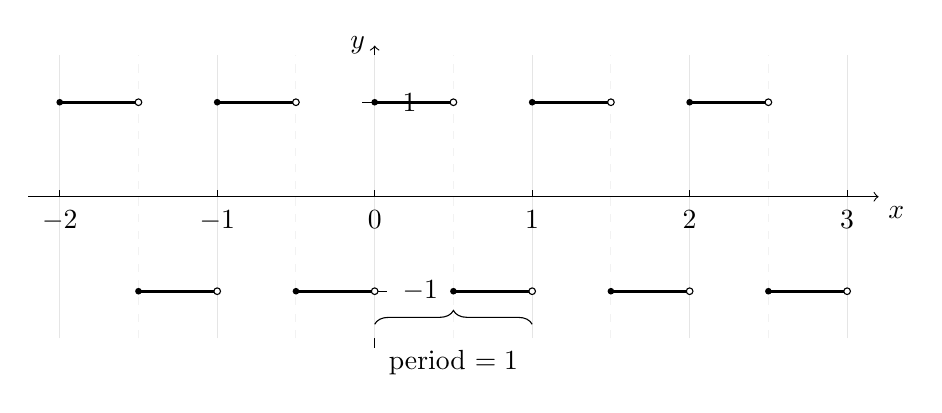
\begin{tikzpicture}[x=2cm,y=1.2cm]

% axes
\draw[->] (-2.2,0) -- (3.2,0) node[below right] {$x$};
\draw[->] (0,-1.6) -- (0,1.6) node[left] {$y$};

% y-level labels
\draw (-0.08,1) -- (0.08,1) node[right=2pt] {$1$};
\draw (-0.08,-1) -- (0.08,-1) node[right=2pt] {$-1$};

% vertical grid at integers and half-integers (light helpers)
\foreach \k in {-2,-1,0,1,2,3}{
  \draw[gray!20] (\k,-1.5) -- (\k,1.5);
}
\foreach \k in {-1.5,-0.5,0.5,1.5,2.5}{
  \draw[gray!10,dashed] (\k,-1.5) -- (\k,1.5);
}

% integer tick labels
\foreach \k in {-2,-1,0,1,2,3}{
  \draw (\k,0) -- (\k,0.07) node[below=4pt] {$\k$};
}

% the square wave: draw for n = -2,...,2
\foreach \n in {-2,-1,0,1,2}{
  % top half: [n, n+1/2) -> y=1
  \draw[line width=1pt] (\n,1) -- (\n+0.5,1);
  % bottom half: [n+1/2, n+1) -> y=-1
  \draw[line width=1pt] (\n+0.5,-1) -- (\n+1,-1);

  % endpoints: closed at left, open at right for each half-interval
  % top half endpoints
  \fill (\n,1) circle (1.2pt); % closed at left
  \draw[fill=white] (\n+0.5,1) circle (1.2pt); % open at right
  % bottom half endpoints
  \fill (\n+0.5,-1) circle (1.2pt); % closed at left
  \draw[fill=white] (\n+1,-1) circle (1.2pt); % open at right
}

% legend for one period
\draw[decorate,decoration={brace,amplitude=5pt}] (0,-1.35) -- (1,-1.35)
  node[midway,below=6pt] {period $=1$};

% labels for pieces
%\node[above right] at (-1.8,1) {$f(x)=1$ on $[n,n+\tfrac12)$};
%\node[below right] at (-1.8,-1) {$f(x)=-1$ on $[n+\tfrac12,n+1)$};

\end{tikzpicture}
  
\end{problem}

\begin{proof}
    First, we define $f_n$ on $[0,1]$, then extend $f_n$ to all of $\mathbb{R}$ by making it 1-periodic. Fix $n$, define $f_n$ by 
    \[
        f_n(x) = 
        \begin{cases}
            (48763n)x & \text{if } x \in [0, \frac{1}{48763n}), \\
            1         & \text{if } x \in [\frac{1}{48763n}, \frac{1}{2} - \frac{1}{48763n}), \\
            1 - (48763n)\cdot(x - (\frac{1}{2} - \frac{1}{48763n})) & \text{if }x \in [\frac{1}{2} - \frac{1}{48763n}, \frac{1}{2} + \frac{1}{48763n}), \\
            -1         & \text{if } x \in [\frac{1}{2} + \frac{1}{48763n}, 1 - \frac{1}{48763n}), \\
            -1 + (48763n) \cdot (x - (1 - \frac{1}{48763n})) & \text{if } x \in [1 - \frac{1}{48763n}, 1)
        \end{cases}
    \]
    For each of these piecewise-defined functions, every piece is continuous, and at each endpoint $x$ the left-hand and right-hand limit value are same and equal to $f_n(x)$. Hence the function is continuous on its whole domain, so $f_n$ is continuous.

    Then we show that $f_n$ converges in $L^2$ to the square wave function, we want to show that
    \[
    \left\|f_n - f\right\|_{L^2([0,1])}^2 = \int_0^1 \left|f_n(x) - f(x)\right|^2 \, dx \longrightarrow 0 .
    \]
    \[
    \begin{aligned}
    \int_0^1 \left|f_n(x) - f(x)\right|^2 \, dx &= 
    \int_0^{\frac{1}{2}} \left|f_n(x) - 1\right|^2 \, dx + \int_{\frac{1}{2}}^{1} \left|f_n(x) + 1\right|^2 \, dx \\
    &= \int_0^{\frac{1}{48763n}} \left|f_n(x) - 1\right|^2 \, dx+ \int_{\frac{1}{2}-\frac{1}{48763n}}^{\frac{1}{2}} \left|f_n(x) - 1\right|^2 \, dx\\
    &+ \int_{\frac{1}{2}}^{\frac{1}{2}+\frac{1}{48763n}} \left|f_n(x) + 1\right|^2\, dx + \int_{1-\frac{1}{48763n}}^{1} \left|f_n(x) + 1\right|^2 \, dx\\
    &= 4 \cdot \frac{1}{3 \cdot 48763n} \to 0 \quad \text{as } n \to \infty 
    \end{aligned}
    \]
    So we can conclude that $f_n$ converges in $L^2$ to the square wave function.
\end{proof}

\begin{problem}[15 pts]
    \vphantom{text}
    \begin{itemize}
        \item [(a)] Evaluate 
    \[
    S_n(\theta) = \sum_{k=1}^{n} \sin(k\theta).
    \]

    \item [(b)] Show that 
    \[
    |S_n(\theta)| \le \pi \varepsilon^{-1}
    \qquad \text{on } [\varepsilon,\, 2\pi - \varepsilon] \text{ for all } n \ge 1.
    \]
    \end{itemize}
\end{problem}

\begin{proof}[(a)]
    We will use the sum-to-product formulas (和差化積公式) that
    \[
        2\sin A \sin B = \cos(A-B) - \cos(A +B)
    \]
    and
    \[
        \cos A - \cos B = -2 \sin (\frac{A+B}{2}) \sin (\frac{A-B}{2})
    \]
    to help us solve the problem. \\
    First, we multiply $2 \sin (\frac{\theta}{2})$ for both sides, and use the formulas above to simplify.
    \[
    \begin{aligned}
        2 \sin (\frac{\theta}{2}) S_n(\theta) &= \sum_{k=1}^{n}2 \sin (k\theta)\sin(\frac{\theta}{2}) \\
        &= \sum_{k=1}^{n} \left( \cos(k\theta-\frac{\theta}{2}) - \cos(k\theta+\frac{\theta}{2})\right) \\
        &= \left(\cos(\frac{\theta}{2}) - \cos(\frac{3\theta}{2})\right) + \dots + \left( \cos(n\theta-\frac{\theta}{2}) - \cos(n\theta+\frac{\theta}{2})\right) \\
        &= \cos(\frac{\theta}{2}) - \cos(n\theta+\frac{\theta}{2}) \\
        &= -2 \sin(\frac{(n+1) \theta}{2}) \sin( \frac{-n \theta}{2}) \\
        &= 2 \sin(\frac{(n+1) \theta}{2}) \sin( \frac{n \theta}{2})
    \end{aligned}
    \]
    And hence when $\sin (\frac{\theta}{2}) \ne 0$, 
    \[
        S_n (\theta) = \frac{\sin(\frac{(n+1) \theta}{2}) \sin( \frac{n \theta}{2})}{\sin (\frac{\theta}{2})},
    \]
    and when $\sin (\frac{\theta}{2}) = 0$, for all integer $k$, $\sin (k \theta) = 0$, and hence $S_n(\theta) = 0$ when $\sin (\frac{\theta}{2}) = 0$.
\end{proof}

\begin{proof}[b]
    From (a), we know for all $n \ge 1$
    \[
        \left \vert S_n (\theta) \right \vert  = \left \vert \frac{\sin(\frac{(n+1) \theta}{2}) \sin( \frac{n \theta}{2})}{\sin (\frac{\theta}{2})} \right \vert \le \frac{1}{\left \vert \sin (\frac{\theta}{2})\right \rvert }
    \]
    For $\theta \in [ \varepsilon, 2 \pi - \varepsilon]$, $\frac{\theta}{2} \in [ \frac{\varepsilon}{2}, \pi - \frac{\varepsilon}{2}] \subset (0, \pi)$. \\
    On $[0, \pi]$, the $\sin$ function attains its minimum on this interval at the endpoint, and $\sin(\frac{\varepsilon}{2}) = \sin(\pi - \frac{\varepsilon}{2})$, and hence
    \[
        \left \vert \sin (\frac{\theta}{2})\right \rvert  \ge \sin (\frac{\varepsilon}{2})
    \]
    Since $\varepsilon \le \pi$, $\frac{\varepsilon}{2} \le \frac{\pi}{2}$, and using the concavity of $\sin$ function on $[0, \frac{\pi}{2}]$, we can get
    \[
        \sin (\frac{\varepsilon}{2}) \ge \frac{1-0}{\frac{\pi}{2}-0} \cdot \frac{\varepsilon}{2} = \frac{\varepsilon}{\pi},
    \]
    and hence
    \[
         \left \vert S_n (\theta) \right \vert \le \frac{1}{\left \vert \sin (\frac{\theta}{2})\right \rvert } \le \frac{1}{\sin (\frac{\varepsilon}{2})} \le \frac{1}{\frac{\varepsilon}{\pi}} = \pi \varepsilon^{-1}
    \]
    And we done.
\end{proof}

\begin{problem}[15 pts]
    Let $f, g \in C(\mathbb{R}/\mathbb{Z}; \mathbb{R})$.  
We define their \emph{periodic convolution} $f * g : \mathbb{R} \to \mathbb{R}$ by
$$
(f * g)(x) := \int_{0}^{1} f(y)\, g(x-y)\, dy.
$$ Prove that $(f * g)$  is smooth whenever $f$ is smooth.
(Remark: A function is called smooth if it has derivatives of all orders.)
\end{problem}
\begin{proof}
      Fix \(x \in \mathbb{R} \), then 
  \begin{align*}
    (f * g)(x) &= \int _0^1 f(y) g(x - y) \, \mathrm{d} y = \int _x^{x-1} f(x - t) g(t) \, (- \mathrm{d} t ) = \int _{x-1}^x f(x - t) g(t) \, \mathrm{d} t \\
    &= \int _0^1 f(x - t) g(t) \, \mathrm{d} t.   
  \end{align*} 
  Now consider 
  \begin{align*}
    \lim_{h \to 0} \frac{(f * g)(x + h) - (f * g)(x)}{h} &= \lim_{h \to 0} \int _0^1 \frac{f(x+h - t) g(t) - f(x - t) g(t)}{h} \, \mathrm{d} t \\
    &= \lim_{h \to 0} \int _0^1 \left( \frac{f(x + h - t) - f(x - t)}{h} \right) g(t) \, \mathrm{d} t.   
  \end{align*}
  Suppose \(\phi _h: \mathbb{R} \to \mathbb{R} \) where 
  \[
    \phi _h(t) = \left( \frac{f(x + h - t) - f(x - t)}{h} \right) g(t),
  \]
  then we claim that \(\left\{ \phi _{\frac{1}{n}}(t) \right\}_{n = 1}^{\infty} \to f^{\prime} (x - t) g(t)\) uniformly, and if we can prove this, then we know
  \begin{align*}
     (f * g)(x)^{\prime} &= \lim_{h \to 0} \frac{(f * g)(x + h) - (f * g)(x)}{h} = \lim_{h \to 0} \int _0^1 \frac{f(x+h - t) g(t) - f(x - t) g(t)}{h} \, \mathrm{d} t \\ &= \lim_{h \to 0} \int _0^1 \phi _h(t) \, \mathrm{d} t = \lim_{n \to \infty} \int _0^1 \phi _{\frac{1}{n}}(t) \, \mathrm{d} t = \int _0^1 \lim_{n \to \infty} \phi _{\frac{1}{n}}(t) \, \mathrm{d} t = \int _0^1 f^{\prime} (x - t) g(t) \, \mathrm{d} t \\ &= \left( f^{\prime} * g \right)(x).  
  \end{align*} 
  Now if we have this, then since the above argument is true for all \(x \in \mathbb{R} \), so \(f * g\) is differentiable at every \(x \in \mathbb{R} \), and since \(f^{\prime} \) is also smooth, so we can repeat this argument to show that \(f * g\) is smooth. Now we prove the claim. For any \(\varepsilon > 0\), we want to show that there exists \(N > 0\) s.t. \(n \ge N\) implies 
  \[
    \left\vert \left( \frac{f \left( x + \frac{1}{n} - t \right) - f(x - t)}{\frac{1}{n}} - f^{\prime}(x - t)  \right) g(t) \right\vert = \left\vert \phi _{\frac{1}{n}}(t) - f^{\prime} (x-t) g(t) \right\vert < \varepsilon \quad \forall t \in [0, 1]. 
  \]    
  However, since 
  \[
    f^{\prime} (x - t) = \lim_{h \to 0} \frac{f(x - t + h) - f(x - t)}{h}, 
  \]
  so there exists \(\delta > 0\) s.t. \(\vert h \vert < \delta  \) implies 
  \[
    \left\vert \frac{f(x - t + h) - f(x - t)}{h} - f^{\prime} (x - t) \right\vert < \frac{\varepsilon}{M}, 
  \]  
  where \(M = \sup _{t \in [0, 1]} \vert g(t) \vert \) (here we suppose \(M > 0\)). Now since there exists \(N_1 > 0\) s.t. \(\frac{1}{N_1} < \delta \), so for all \(n \ge N_1\) we have \(\frac{1}{n} \le \frac{1}{N_1} < \delta \) and we have 
  \begin{align*}
    \left\vert \left( \frac{f \left( x + \frac{1}{n} - t \right) - f(x - t)}{\frac{1}{n}} - f^{\prime}(x - t)  \right) g(t) \right\vert &< \left\vert \frac{\varepsilon}{M} g(t) \right\vert \le \left\vert \frac{\varepsilon}{M} \cdot M \right\vert = \varepsilon,
  \end{align*}     
  and we're done. Now if \(M = 0\), then \(g(t) = 0\) on \([0, 1]\) and thus we also have 
  \[
    \left\vert \left( \frac{f \left( x + \frac{1}{n} - t \right) - f(x - t)}{\frac{1}{n}} - f^{\prime}(x - t)  \right) g(t) \right\vert = 0 < \varepsilon.
  \]  
  Hence, in either case we can show the claim is true.
\end{proof}
\cofeCm{0.5}{1}{180}{0}{0}

